\begin{frame}
\setbeamercovered{invisible}
\frametitle{Spin-Dipole Oscillation: dynamic measurement}

\centering
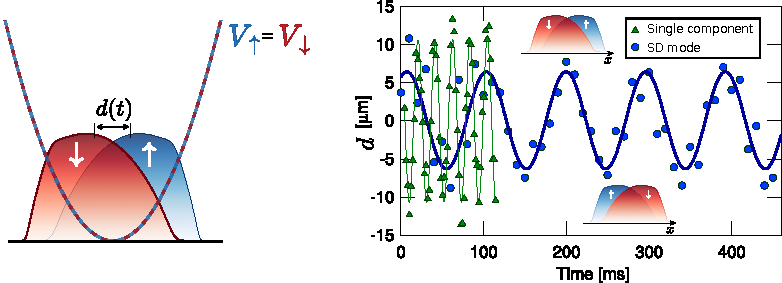
\includegraphics[width=0.95\linewidth]{Figures/SD_Oscillations2.pdf}

\begin{itemize}
\item We measure $\omega_{\text{SD}}/\omega_x = 0.218(2)$
	\begin{itemize}
	\item LDA $\omega_{\text{SD}} = 0.189(15) \omega_x$
	\item GPE $\omega_{\text{SD}} = 0.213(17) \omega_x$ 
	\end{itemize}
\item Sum rule approach links polarizability $\mathcal P$ and SD mode frequency $\omega_{\text{SD}}$: 
\begin{equation*}
\omega_{\text{SD}} = \frac{1}{\sqrt \mathcal P} \omega_x
\end{equation*}
%\item LDA prediction: 
%\begin{equation*}
%\omega_{\text{SD}} = \sqrt{\frac{a-a_{\uparrow\downarrow}}{a+a_{\uparrow\downarrow}}} \omega_x
%\end{equation*}
\end{itemize}

\end{frame}
